\addcontentsline{toc}{chapter}{Занятие 12. Числовые характеристики случайных величин II}
\chapter*{Занятие 12. Числовые характеристики случайных величин II}

\addcontentsline{toc}{section}{Контрольные вопросы и задания}
\section*{Контрольные вопросы и задания}

\subsubsection*{Запишите основные вероятностные распределения и поясните смысл их параметров.}

Основные распределения:
\begin{enumerate}
\item дискретное распределение:
\begin{enumerate}
\item равномерное дискретное распределение
$$P \left( \xi = k \right) =
\frac{1}{N},
1 \leq k \leq N,
M \xi = \frac{N+1}{2}, D \xi = \frac{N^2 - 1}{12};$$
\item биномиальное распределение: $ \xi \sim Biom \left( n, p \right) $
$$P \left\{ \xi = k \right\} =
C_n^k p^k q^{n-k},$$
где $0 \leq k \leq n, q = 1 - p, M \xi = np, D \xi = npq$;
\item геометрическое распределение $ \xi \sim Geom \left( p \right), p \in \left( 0, 1 \right) $
$$P \left\{ \xi = k \right\} =
pq^k,
k \geq 0,
M \xi = \frac{q}{p},
D \xi = \frac{q}{p^2};$$
\item пуассоновское распределение: $ \xi \sim Pois \left( \lambda \right), \lambda > 0$
$$P \left\{ \xi = k \right\} = \frac{ \lambda^k}{k!} \cdot e^{- \lambda },
k \geq 0,
M \xi = \lambda,
D \xi = \lambda;$$
\end{enumerate}
\item непрерывные распределения:
\begin{enumerate}
\item равномерное распределение: $ \xi \sim U \left( \left[ a, b \right] \right) $
$$p \left( x \right) =
\begin{cases}
\frac{1}{b-a}, \qquad x \in \left[ a, b \right], \\
0, x \notin \left[ a, b \right], \\
\end{cases}
M \xi = \frac{a+b}{2},
D \xi = \frac{ \left( b-a \right)^2}{12};$$
\item экспоненциальное распределение: $ \xi \sim Exp \left( \lambda \right), \lambda > 0$
$$p \left( x \right) =
\begin{cases}
\lambda e^{- \lambda x}, \qquad x \geq 0, \\
0, \qquad x < 0, \\
\end{cases}
M \xi = \frac{1}{ \lambda },
D \xi = \frac{1}{ \lambda^2};$$
\item распределение Коши: $ \xi \sim C \left( \Theta \right), \Theta > 0$
$$p \left( x \right) =
\frac{ \Theta }{ \pi \left( x^2 + \Theta^2 \right) };$$
\item гауссовское (нормальное) распределение:
$$ \xi \sim \mathcal{N} \left( a, \sigma^2 \right),
a \in \mathbb{R},
\sigma^2 > 0,$$
$$p \left( x \right) = \frac{1}{ \sqrt{2 \pi } \cdot \sigma } \cdot e^{- \frac{ \left( x-a \right)^2}{2 \sigma^2}},
x \in \mathbb{R},
M \xi = a,
D \xi = \sigma^2.$$
\end{enumerate}
\end{enumerate}

\subsubsection*{Сформулируйте основные свойства математического ожидания и дисперсии.}

Свойства математического ожидания:
\begin{enumerate}
\item если $ \exists M$, то $ \forall c \in \mathbb{R} \, \exists M \left( c \xi \right) $ и $ M \left( c \xi \right) = cM \xi $;
\item если существует $M \xi $ и $M \eta $, то $ \exists M \left( \xi + \eta \right) $ и $M \left( \xi + \eta \right) = M \xi + M \eta $.
Из этих двух условий следует, что математическое ожидание является линейной функцией;
\item $ \exists M \xi \iff \exists M \left| \xi \right| $, и кроме того $ \left| M \xi \right| \leq M \left| \xi \right| $;
\item если $ \xi \geq 0$, то $M \xi \geq 0$;
\item $\xi \geq \eta, \, \exists \xi, \, \exists \eta \Rightarrow M \xi \geq M \eta $;
\item если $ \eta $ и $ \xi $ --- независимые случайные величины,
для которых существует математическое ожидание, то $ \exists M \left( \xi \eta \right) = M \xi \cdot M \eta $.
\end{enumerate}

Свойства дисперсии:
\begin{enumerate}
\item $D \xi \geq 0$'
\item $ \forall \lambda \in \mathbb{R}: \qquad D \left( \lambda \xi \right) = \lambda^2 D \xi $;
\item для независимых $ \eta $ и $ \xi \, D \left( \xi + \eta \right) = D \xi + D \eta $.
\end{enumerate}

\addcontentsline{toc}{section}{Аудиторные задачи}
\section*{Аудиторные задачи}

\subsubsection*{12.4}

\textit{Задание.} Существует $n$ типов игрушек, которые можно найти в конфете <<Киндер-сюрприз>>.
Сколько в среднем нужно перебрать конфет, чтобы набрать полную коллекцию?
Как ведёт себя количество попыток при $n \to \infty $?

\textit{Решение.} Количество игрушек не ограничено.
Сколько бы их не брали, общее количество от этого не изменится.
Все игрушки одинаково равномерно перемешаны, так что каждый тип встречается с одинаковой вероятностью $1/n$.

Вероятность в формуле 
$$M \xi =
\sum \limits_{k=0}^{ \infty } kP \left( \xi = k \right) $$
будет найти сложно, поэтому пользуемся формулой
$$M \xi =
\sum \limits_{k=0}^{ \infty } P \left( \xi > k \right).$$

Обозначим через $ \xi $ наименьшее количество конфет, которые необходимо купить, чтобы получить полный набор игрушек,
то есть каждый тип из $n$ типов игрушек должен быть там представлен. 
Напишем такое событие $ \left\{ \xi > k \right\} $.
Оно означает, что среди $k$ игрушек ещё нет полного набора.

$P \left( \xi > k \right) = P$(среди $k$ игрушек нет полного набора) $= P$(среди $k$ игрушек не хватает хотя бы одного типа).
Используем формулу включений-исключений.
Введём события $A_i^k =$ {нет $i$-того типа среди $k$ игрушек}.
Через эти события запишем формулу включений-исключений
$P \left( \xi > k \right) = \\
= P \left( A_1^k \right) C_n^1 -
C_n^2 P \left( A_1^k \cap A_2^k \right) +
C_n^3 \cdot P \left( A_1^k \cap A_2^k \cap A_3^k \right) -
\dotsc + \\
+ \left( -1 \right)^n P \left( A_1^k \cap A_2^k \cap \dotsc \cap A_{n-1}^k \right) C_n^{n-1}$.
Не может быть такого, что нет ни одного типа.
Вычисляем $P \left( A_1^k \right) = P$(среди $k$ игрушек нет игрушек первого типа) =
\begin{equation*}
\begin{split}
= \sum \limits_{m_2 + m_3 + \dotsc + m_n = k, m_i \geq 0} \frac{k!}{m_2! \dotsc m_n!} \cdot \left( \frac{1}{n} \right)^{m_2} \left( \frac{1}{n} \right)^{n_3} \cdot \dotsc \cdot \left( \frac{1}{n} \right)^{m_n} = \\
= \left( \frac{1}{n} \right)^k \left( n-1 \right)^k =
\left( 1 - \frac{1}{n} \right)^k.
\end{split}
\end{equation*}

Вычисляем $P \left( A_1^k \cap A_2^k \right) = P$(среди $k$ игрушек нет первого и второго типов игрушек) =
\begin{equation*}
\begin{split}
= \sum \limits_{m_3 + m_4 + \dotsc + m_n = k, m_i \geq 0} \frac{k!}{m_3! \dotsc m_n!} \cdot
\left( \frac{1}{n} \right)^{m_3} \left( \frac{1}{n} \right)^{m_4} \cdot \dotsc \cdot \left( \frac{1}{n} \right)^{m_n} = \\
= \left( \frac{1}{n} \right)^k \left( n-2 \right)^k =
\left( 1 - \frac{2}{n} \right)^k.
\end{split}
\end{equation*}

В формуле используется мультибиномиальное распределение
$$C_k^{m_1} C_{k-m_1}^{m_2} C_{k- m_1 - m_2}^{m_3} \dotsc.$$

Будем пользоваться формулой
\begin{equation*}
\begin{split}
M \xi =
\sum \limits_{k=0}^{ \infty } P \left( \xi > k \right) =
C_n^1 \sum \limits_{k=0}^{ \infty } P \left( A_1^k \right) -
C_n^2 \sum \limits_{k=0}^{ \infty } P \left( A_1^k \cap A_2^k \right) +
\dotsc + \\
+ \left( -1 \right)^n C_n^{n-1} \sum \limits_{k=0}^{ \infty } P \left( A_1^k \cap A_2^k \cap \dotsc \cap A_{n-1}^k \right),
\end{split}
\end{equation*}
где
\begin{equation*}
\begin{split}
\sum \limits_{k=0}^{ \infty } P \left( A_1^k \right) =
\sum \limits_{k=0}^{ \infty } \left( 1 - \frac{1}{n} \right)^k =
\frac{1}{1 - \left( 1 - \frac{1}{n} \right) } =
n,
\sum \limits_{k=0}^{ \infty } P \left( A_1^k \cap A_2^k \right) =
\frac{n}{2}, \\
\sum \limits_{k=0}^{ \infty } P \left( A_1^k \cap A_2^k \cap \dotsc \cap A_{n-1}^k \right) =
\frac{n}{n-1}.
\end{split}
\end{equation*}
Получаем
$$M \xi =
nC_n^1 - \frac{n}{2} \cdot C_n^2 + \dotsc + \left( -1 \right)^n C_n^{n-1} \cdot \frac{n}{n-1}.$$

\subsubsection*{12.5}

\textit{Задание.} В магазине находится $A$ тонн товара, который быстро портится и который нужно реализовать за один день.
Спрос на этот товар --- случайная величина, которая имеет показательное распределение с параметром $1/2$ (в тоннах).
Цена одного килограмма товара составляет одну гривну.
Найдите:
\begin{enumerate}[label=\alph*)]
\item средний спрос за день;
\item среднюю выручку за день при условии, что $A = 1$;
\item среднюю выручку за день при условии, что $A = 1$, а нереализованный остаток товара утилизируется по 30 коп. за килограмм.
При каком $A$ выручка будет максимальной?
\end{enumerate}

\textit{Решение.} Пусть $ \xi $ --- это спрос на товар ( случайная величина с показательным распределением с параметром $1/2$)
$$ \xi \sim \prod \left( \frac{1}{2} \right).$$

\begin{enumerate}[label=\alph*)]
\item Нужно найти математическое ожидание $ \xi $.
В тоннах оно равно
$$M \xi =
\frac{1}{ \frac{1}{2}} =
2.$$

Это означает, что за день в среднем люди хотели, чтобы было две тонны продукта;
\item введём новую случайную величину.
Пусть $ \eta $ --- выручка за день.
Выразим через $A = 1$ и $ \xi $.
Получим $ \eta = \min \left( A, \xi \right) \cdot 1000 = \min \left( 1, \xi \right) \cdot 1000$ (грн.).

Теперь ищем
\begin{equation*}
\begin{split}
M \eta =
10^3 \cdot M \min \left( \xi, \eta \right) =
10^3 \int \limits_{- \infty }^{+ \infty } \min \left( 1, x \right) p_{ \xi } \left( x \right) dx = \\
= \int \limits_0^{+ \infty } \min \left( 1, x \right) \cdot \frac{1}{2} \cdot e^{- \frac{x}{2}} dx \cdot 10^3.
\end{split}
\end{equation*}
Разобьём на 2 интеграла
$$M \eta =
10^3 \int \limits_0^1 x \cdot \frac{1}{2} \cdot e^{- \frac{x}{2}} dx + 10^3 \int \limits_1^{+ \infty } \frac{1}{2} \cdot e^{- \frac{x}{2}} dx.$$
Вычисляем каждый интеграл отдельно.
Первый интеграл берём по частям
$$u = x, dv = e^{- \frac{x}{2}} dx, du = dx, v = \int e^{- \frac{x}{2}} dx = -2 \int e^{- \frac{x}{2}} d \left( - \frac{x}{2} \right) = -2e^{- \frac{x}{2}}.$$
Получаем
\begin{equation*}
\begin{split}
\int \limits_0^1 x \cdot e^{- \frac{x}{2}} dx =
\left. -2xe^{- \frac{x}{2}} \right|_0^1 + 2 \int \limits_0^1 e^{- \frac{x}{2}} dx =
\left. -2e^{- \frac{1}{2}} + 2 \cdot \left( -2 \right) \cdot e^{- \frac{x}{2}} \right|_0^1 = \\
= -2e^{- \frac{1}{2}} -4e^{- \frac{1}{2}} + 4 =
-6e^{- \frac{1}{2}} + 4.
\end{split}
\end{equation*}
Подставляем
\begin{equation*}
\begin{split}
M \eta =
10^3 \cdot \left( -3e^{- \frac{1}{2}} + 2 \right) + 10^3 \cdot e^{- \frac{1}{2}} =
10^3 \left( 2 - 2e^{- \frac{1}{2}} \right) = \\
= 2 \cdot 10^3 \left( 1 - e^{- \frac{1}{2}} \right) =
2000 \left( 1 - e^{- \frac{1}{2}} \right).
\end{split}
\end{equation*}
Выражение в скобках меньше чем $1/2$, поэтому $M \xi < 1000$;

\item ищем среднюю выручку за день при условии, что $A = 1$, а нереализованный остаток товара утилизируется по 30 коп. за килограмм.
Введём $ \zeta = \min \left( 1, \xi \right) \cdot 1000 + \left[ 1 - \min \left( 1, \xi \right) \right] \cdot 300$.
Перегруппируем слагаемые $ \zeta = \min \left( 1, \xi \right) \cdot 1000 + 300 - 300 \cdot \min \left( 1, \xi \right) $.
Вынесем $ \min \left( 1, \xi \right) $ за скобки $ \zeta = 700 \cdot \min \left( 1, \xi \right) + 300$.
Из предыдущего пункта
$$M \zeta =
2 \cdot 700 \left( 1 - e^{- \frac{1}{2}} \right) + 300.$$

Выгода будет максимальной, если товар не будет оставаться не проданным.
Так как средний спрос на товар --- 2 тонны, то и в магазине должно находиться $A = 2$ тонны товара.
\end{enumerate}

\subsubsection*{12.6}

\textit{Задание.} На фрезеровочный станок с конвейера приходит в среднем 5 деталей.
Время от времени станок требует налаживания, и тогда его останавливают в среднем на 15 минут.
Найдите математическое ожидание числа деталей, которые поступают на станок за время его простоя.

\textit{Решение.}
Введём случайные величины $ \xi_i$ --- количество деталей,
которые пришли с конвейера за $i$-тую минуту простоя, $ \nu $ --- это время простоя, то есть целое количество минут.

Тогда $ \eta $ --- количество деталей, которые поступили за время простоя.
Это
$$M \eta =
M \left( \sum \limits_{i=1}^{ \nu } \xi_i \right) =
M \nu \cdot M \xi_1.$$

По условию $M \xi_i = 5, \xi_i \geq 0, M \nu = 15$.
Тогда $M \eta = 15 \cdot 5 = 75$.

\subsubsection*{12.7}

\textit{Задание.} Количество печатных ошибок в книге имеет распределение Пуассона с параметром $ \lambda > 0$.
Найдите математическое ожидание количества ошибок после трёх независимых корректорских проверок, если при каждой проверке каждая из ошибок исправляется с вероятностью $p$.

\textit{Решение.} Целесообразно ввести такие случайные величины.
Пусть $ \xi $ --- начальное количество ошибок.
Она имеет распределение Пуассона
$$P \left\{ \xi = k \right\} =
\frac{ \lambda^k}{k!} \cdot e^{- \lambda },$$
где $k = 0, 1, \dotsc $.

Пусть $ \xi_i$ --- количество ошибок после $i$-ой корректорской проверки.
Начнём с $ \xi_1$.
По каждой ошибке можем ввести функцию индикатор
$$ \xi_1 = \sum \limits_{i=1}^{ \xi } \mathbbm{1} \left( A \right),$$
где событие $A$ означает, что $i$-тая ошибка корректором не исправлена.
Тогда найдём математическое ожидание
$M \xi_1 = M \xi \cdot M \mathbbm{1}$($i$-тую ошибку корректор не исправил)$= M \xi \cdot M \mathbbm{1}$(первую ошибку корректор не увидел)$= \lambda \left( 1 - p \right) $.
Теперь
$$ \xi_2 =
\sum \limits_{i=1}^{ \xi_1} \mathbbm{1} A.$$

Найдём её математическое ожидание
$M \xi_2 = M \xi_1 \cdot M \mathbbm{1}$(первую ошибку не исправили)
$= M \xi_1 \cdot P$(первую ошибку не исправили)$= \lambda \left( 1-p \right) \left( 1-p \right) = \\
= \lambda \left( 1-p \right)^2$.

Соответственно $M \xi_3 = \lambda \left( 1-p \right)^3.$
Докажем, что $ \xi_1, \xi_2, \xi_3$ тоже имеют распределение Пуассона.

нужно найти гипотезы об ошибках перед проверкой
$$P \left\{ \xi_1 = k \right\} =
\sum \limits_{i=k}^{ \infty } P \left( \xi = i \right) P \left( \left. \xi_1 = k \right| \xi = i \right) $$
--- формула полной вероятности.
$$P \left\{ \xi_1 = k \right\} =
\sum \limits_{i=k}^{ \infty } \frac{ \lambda^i}{i!} \cdot e^{- \lambda } C_i^k p^{i-k} \left( 1-p \right)^k,$$
где $p^{i-k}$ означает, что какие-то $i-k$ ошибки были исправлены.
$$P \left\{ \xi_1 = k \right\} =
e^{- \lambda } \left( 1-p \right)^k \sum \limits_{i=k}^{ \infty } \frac{ \lambda^i}{i!} \cdot \frac{i!}{k! \left( i-k \right)!} \cdot p^{i-k}.$$
Сократим на $i!$ и сделаем замену $i - k = m, i = m + k$.
Получим
\begin{equation*}
\begin{split}
P \left\{ \xi_1 = k \right\} =
\frac{e^{- \lambda } \left( 1-p \right)^k}{k!} \sum \limits_{m=0}^{ \infty } \lambda^{m+k} \cdot \frac{p^m}{m!} =
\frac{e^{- \lambda } \lambda^k \left( 1-p \right)^k}{k!} \sum \limits_{m=0}^{ \infty } \frac{ \lambda^m}{m!} \cdot p^m = \\
= e^{- \lambda } \cdot \frac{ \lambda^k \left( 1-p \right)^k}{k!} \cdot e^{ \lambda p} =
\frac{e^{- \lambda \left( 1-p \right) } \left( \lambda \left( 1-p \right) \right)^k}{k!}
\end{split}
\end{equation*}
--- распределение Пуассона с параметром $ \lambda \left( 1-p \right) $.

Аналогично для $ \xi_2, \xi_3$.
Делаем для них соответствующие гипотезы.

\subsubsection*{12.8}

\textit{Задание.}
Эволюция элементарных частиц некоторого типа происходит следующим образом;
каждая частица живёт одну секунду, после окончания которой делится на две с вероятностью $2/3$ или исчезает с вероятностью $1/3$.
Потом каждый из её потомков, независимо от других, делится на две части с вероятностью $2/3$ или исчезает с вероятностью $1/3$ и т.д.
Вычислите математическое ожидание количества частиц через:
\begin{enumerate}[label=\alph*)]
\item 2 секунды;
\item 10 секунд, при условии, что в начальный момент времени была одна частица.
\end{enumerate}

\textit{Решение.} Введём $ \xi_n$ --- количество частиц в $n$-тый момент времени, в данном случае на $n$-той секунде.
Знаем, что $ \xi_0 = 1$, то есть в начальный момент времени была одна частичка.
Найдём рекуррентную формулу
$$ \xi_{n+1} = \sum \limits_{i=1}^{ \xi_n} \mathbbm{1} \left( A \right) \cdot 2,$$
где событие $A$ означает, что $i$-тая частица поделилась на две, а 2 --- количество потомков.

Тогда $M \xi_{n+1} = M \xi_n \cdot M \mathbbm{1}$(частица поделилась на две)$ \cdot 2 = M \xi_n \cdot P$(частица поделилась на две)$ \cdot 2 =$
$$= \frac{4}{3} \cdot M \xi_n =
\left( \frac{4}{3} \right)^2 \cdot M \xi_{n-1} =
\dotsc =
\left( \frac{4}{3} \right)^{n+1} M \xi_0 =
\left( \frac{4}{3} \right)^{n+1} \cdot 1 =
\left( \frac{4}{3} \right)^{n+1}.$$

\begin{enumerate}[label=\alph*)]
\item Через две секунды
$$M \xi_2 =
\left( \frac{4}{3} \right)^2 =
\frac{16}{9};$$
\item через 10 секунд
$$M \xi_{10} =
\left( \frac{4}{3} \right)^{10}.$$
\end{enumerate}

\addcontentsline{toc}{section}{Домашнее задание}
\section*{Домашнее задание}

\subsubsection*{12.11}

\textit{Задание.} Время безотказной работы подшипника --- случайная величина, которая имеет показательное распределение с параметром $ \alpha = 1$ (в годах).
После одного года эксплуатации или же при выходе из строя подшипник заменяют на новый.
Найдите математическое ожидание времени службы подшипника.

\textit{Решение.} Пусть $ \xi $ --- случайная величина, которая характеризует время работы подшипника.
По условию она имеет показательное распределение
$p \left( x \right) =
\alpha e^{- \alpha x} \cdot \mathbbm{1} \left( x \geq 0 \right) =
e^{-x} \cdot \mathbbm{1} \left( x \geq 0 \right) $.
Введём новую случайную величину.
Пусть $ \eta  = \min \left( 1, \xi \right) $ --- время работы подшипника до замены или поломки.
Найдём её математическое ожидание
$$M \eta =
\int \limits_{- \infty }^{+ \infty } \min \left( 1, x \right) p \left( x \right) dx =
\int \limits_{- \infty }^{+ \infty } \min \left( 1, x \right) e^{-x} \cdot \mathbbm{1} \left( x \geq 0 \right).$$
Учтём индикатор в пределах интегрирования
$$M \eta =
\int \limits_0^{+ \infty } \min \left( 1, x \right) e^{-x} dx =
\int \limits_0^1 xe^{-x} dx + \int \limits_1^{+ \infty } e^{-x} dx.$$
Берём первый интеграл по частям
$$u = x,
dv = e^{x}dx,
du = dx, 
v = \int e^{-x} dx = -e^{-x}.$$
Подставляем
$$M \eta =
\left. xe^{-x} \right|_0^1 + \int \limits_0^1 e^{-x} dx - \left. e^{-x} \right|)1^{+ \infty } =
-1 \cdot e^{-1} - \left. e^{-x} \right|_0^1 - e^{- \infty } + e^{-1}.$$
Экспонента на $- \infty $ принимает значение 0, поэтому
$$M \eta = 
- \frac{1}{e} - e^{-1} + e^0 + \frac{1}{e} =
1 - \frac{1}{e}.$$

\subsubsection*{12.12}

\textit{Задание.} Вероятность выиграть в компьютерную игру равна $1/4$.
Количество попыток, которые можно сделать, равна 4.
Найдите количество попыток, которые будут сделаны, если при выигрыше игры прекращаются.

\textit{Решение.} Введём случайную величину $ \xi = \left\{ 1, 2, 3, 4 \right\} $ --- это количество попыток до прекращения игр.
Построим для неё график функции распределения.

Найдём вероятность $P \left\{ \xi \leq 4 \right\} = F_{ \xi } \left( 4 \right) = 1$, так как по условию всего даётся 4 попытки, после которых игры прекращаются.
$$P \left\{ \xi \leq 1 - 0 \right\} =
F_{ \xi } \left( 1 - 0 \right) =
0,$$
так как выиграть можно минимум с первой попытки.
По условию
$$P \left\{ \xi \leq 1 \right\} =
F_{ \xi } \left( 1 \right) =
\frac{1}{4}.$$
Ищем вероятность того, что $ \xi $ будет равна двум
$$P \left\{ \xi = 2 \right\} =
\frac{1}{4} \cdot \left( 1 - \frac{1}{4} \right) =
\frac{1}{4} \cdot \frac{3}{4} =
\frac{3}{16},$$
а вероятность того, что $ \xi $ будет равна трём, равна
$$P \left\{ \xi = 3 \right\} =
\frac{1}{4} \cdot \left( \frac{3}{4} \right)^2 =
\frac{1}{4} \cdot \frac{9}{16} =
\frac{9}{64}.$$
Из этого следует, что функция распределения равна
$$F_{ \xi } \left( 2 \right) =
P \left\{ \xi \leq 2 \right\} =
P \left\{ \xi = 1 \right\} + P \left\{ \xi = 2 \right\} =
\frac{1}{4} + \frac{3}{16} =
\frac{7}{16}.$$
В точке 3 получаем
$$F_{ \xi } \left( 3 \right) =
P \left\{ \xi \leq 3 \right\} =
P \left\{ \xi \leq 2 \right\} + P \left\{ \xi = 3 \right\} =
\frac{7}{16} + \frac{9}{64} =
\frac{28+9}{64} =
\frac{37}{64}.$$

Изображаем функцию распределения на рисунке \ref{fig:1212}.

\begin{figure}[h!]
  \centering
  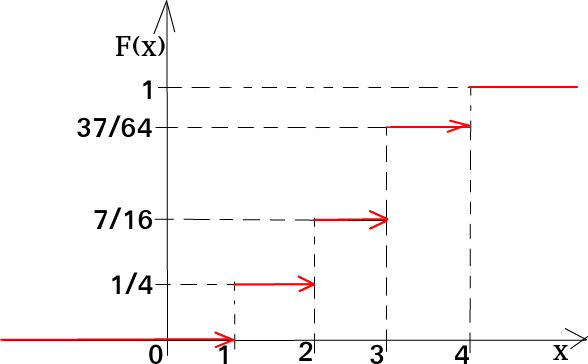
\includegraphics[width=1\textwidth]{./pictures/12_12.png}
  \caption{Функция распределения случайной величины $ \xi $}
  \label{fig:1212}
\end{figure}

Найдём математическое ожидание данной случайной величины
$$M \xi =
\sum \limits_{k=1}^4 k \cdot P \left\{ \xi = k \right\} =
\sum \limits_{k=1}^4 k \cdot p \left( 1-p \right)^{k-1}.$$
Подставим известные значения.
При $k = 4$ вероятность успеха будет равна 1, так как это последняя попытка, на которой можно и выиграть, и проиграть.
При этом игра закончится
$$M \xi =
1 \cdot \frac{1}{4} \left( \frac{3}{4} \right)^0 +
2 \cdot \frac{1}{4} \left( \frac{3}{4} \right)^1 +
3 \cdot \frac{1}{4} \left( \frac{3}{4} \right)^3 +
4 \cdot \left( \frac{1}{4} + \frac{3}{4} \right) \left( \frac{3}{4} \right)^3.$$
Упростим слагаемые
$$M \xi =
\frac{1}{4} + \frac{1}{16} + \frac{27}{64} + \frac{4 \cdot 27}{64} =
\frac{40+135}{64} =
\frac{175}{64} \approx
2.7$$

\subsubsection*{12.13}

\textit{Задание.} Математик имеет связку $n$ ключей, один из которых подходит к замку.
Математик случайным образом испытывает ключи, пока один из них не подойдёт к замку.
Найдите математическое ожидание и дисперсию количества испытаний, если после каждого испытания ключ:
\begin{enumerate}[label=\alph*)]
\item возвращается;
\item не возвращается в связку.
\end{enumerate}

\textit{Решение.}
\begin{enumerate}[label=\alph*)]
\item Обозначим через $ \xi \geq 1$ количество испытаний до первого успеха.
Вероятность того, что ключ подошёл, равна $1/n$.
Тогда вероятность того, что подошёл $k$-тый ключ, равна
$$P \left\{ \xi = k \right\} =
\frac{1}{n} \left( 1 - \frac{1}{n} \right)^{k-1}.$$
Имеем геометрическое распределение с параметром
$$p = \frac{1}{n}.$$
Математическое ожидание при геометрическом распределении равно
$$M \xi =
\frac{1}{p} =
\frac{1}{ \frac{1}{n}} =
n.$$
Дисперсия равна
$$D \xi =
\frac{1-p}{p^2} =
\frac{n-1}{n} \cdot n^2 =
n \left( n-1 \right);$$
\item обозначим через $ \eta \geq 1$ количество попыток до первого успеха.
Вероятность того, что первый ключ подойдёт, равна
$$P \left\{ \eta = 1 \right\} =
\frac{1}{n}.$$
Найдём вероятность того, что подойдёт второй ключ.
При этом первый подойти не должен.
Вероятность того, что первый ключ не подойдёт, равна
$$ \frac{n-1}{n},$$
так как из $n$ ключей $ \left( n-1 \right) $ не подходят к замку.
Остаётся $ \left( n-1 \right) $, 1 из которых подходит к замку. 
Тогда вероятность того, что подойдёт второй ключ, равна
$$P \left\{ \eta = 2 \right\} =
\frac{n-1}{n} \cdot \frac{1}{n-1} =
\frac{1}{n}.$$
Найдём вероятность того, что подойдёт третий ключ.
При этом первый и второй ключи подойти не должны.
Вероятность того, что второй ключ не подойдёт, равна
$$ \frac{n-2}{n-1},$$
так как есть $ \left( n-1 \right) $ ключ, из которых всего 1 подходит, а остальные $ \left( n-2 \right) $ не подходят.
Остаётся $ \left( n-2 \right) $ ключа, один из которых подходит.
По правилу умножения получаем
$$P \left\{ \eta = 3 \right\} =
\frac{n-1}{n} \cdot \frac{n-2}{n-1} \cdot \frac{1}{n-2} =
\frac{1}{n}.$$
Аналогично находим общую формулу для вероятности
$$P \left\{ \eta = k \right\} =
\frac{n-1}{n} \cdot \frac{n-2}{n-1} \cdot \dotsc \cdot \frac{n-k-1}{n-k} \cdot \frac{1}{n-k-1} =
\frac{1}{n}.$$
Ищем математическое ожидание такой случайной величины
$$M \eta =
\sum \limits_{k=1}^n k \cdot \frac{1}{n} =
\frac{1}{n} \sum \limits_{k=1}^n k =
\frac{1}{n} \cdot \frac{1+n}{2} \cdot n =
\frac{n+1}{2}.$$
Ищем второй момент
$$M \eta^2 =
\sum \limits_{k=1}^n k^2 \cdot \frac{1}{n} =
\frac{1}{n} \sum \limits_{k=1}^n k^2 =
\frac{1}{n} \cdot \frac{n \left( n+1 \right) \left( 2n+1 \right) }{6} =
\frac{ \left( n+1 \right) \left( 2n+1 \right) }{6}.$$
Ищем дисперсию
$$D \eta =
M \eta^2 - \left( M \eta \right)^2 =
\frac{ \left( n+1 \right) \left( 2n+1 \right) }{6} - \left( \frac{n+1}{2} \right)^2.$$
Возводим в квадрат второе слагаемое
$$D \eta =
\frac{ \left( n+1 \right) \left( 2n+1 \right) }{6} - \frac{ \left( n+1 \right)^2}{4}.$$
Приводим к общему знаменателю, выносим $ \left( n+1 \right) $ за скобки
$$D \eta =
\frac{ \left( n+1 \right) \left( 4n + 2 - 3n - 3 \right) }{12} =
\frac{ \left( n+1 \right) \left( n-1 \right) }{12} =
\frac{n^2 - 1}{12}.$$
\end{enumerate}

\subsubsection*{12.15}

\textit{Задание.} Иван и Пётр играют в орлянку.
Найдите среднее количество игр, сыгранных до разорения одного из игроков, если Иван имеет три гривны, Пётр --- две гривны, а ставка в каждой игре составляет одну гривну.

\textit{Решение.} Для решения задачи можно использовать метод отражений.
При этом получается бесконечный прямоугольник с двумя диагоналями, которые нельзя пересекать.

Можно поставить задачу следующим образом.
Есть начальное состояние $ \left\{ 3, 2 \right\} $.
Обозначим его через $S$.
Из этого состояния можем перейти в состояние $ \left\{ 4, 1 \right\} $, из которого можно перейти в состояние $ \left\{ 5, 0 \right\} \equiv F$.
Среднее состояние обозначим через $M$.
Из состояния $S$ можем перейти в самого себя (если стало $ \left\{ 2, 3 \right\} $, что то же самое) или в состояние $M$.
Из состояния $M$ можем вернуться в $S$ или перейти в $F$.
В состоянии $F$ игра закончена, так как у одного из игроков осталось 0 гривен, в то время как у другого --- 5 гривен.
Следовательно, из состояния $F$ никуда не переходим.
Это конечное состояние.
Получаем граф, изображённый на рисунке \ref{fig:1215}.

\begin{figure}[h!]
  \centering
  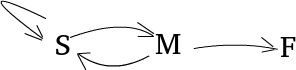
\includegraphics[width=.6\textwidth]{./pictures/12_15.png}
  \caption{Граф}
  \label{fig:1215}
\end{figure}

Нужно найти вероятность пути из $k$ шагов, когда $S$ стоит на первом месте, $F$ стоит на последнем, $M$ не может идти за $M$, а перед $F$ может стоять только $M$.
То есть имеем такую цепочку $S \dotsc SMF$, где всего $k$ элементов.
Можно рассмотреть цепочку $S \dotsc S$ и предположить, что в ней только $S$.
Следующий шаг --- добавить в неё $M$ на какую-то позицию.
Далее добавить 2 $M$, 3 $M$ и так далее.
Но вычислить эти вероятности сложно, так как возникают многомерные фигуры.

Так как есть граф, построим матрицу смежности
$$ \hat{P'} =
\bordermatrix{~ & S & M & F \cr
              S & 1 & 1 & 0 \cr
              M & 1 & 0 & 1 \cr
	      F & 0 & 0 & 0 \cr },$$
где строки указывают, из какой вершины переходим, а столбцы --- в какую.

Всего путей длины $k$ есть $2^k$ штук, так как из каждой вершины можем попасть в две.
Умножим матрицу на $1/2$.
Получим
$$ \hat{P'} =
\bordermatrix{~ & S & M & F \cr
              S & \frac{1}{2} & \frac{1}{2} & 0 \cr
              M & \frac{1}{2} & 0 & \frac{1}{2} \cr
	      F & 0 & 0 & 0 \cr }.$$

Введём обозначение $i \in \left\{ S, M ,F \right\} $.
Вероятность того, что начальное состояние --- это $i$, равна
$$p_{0i} =
\begin{cases}
1, \qquad i = S, \\
0, \qquad i \neq S.
\end{cases}$$
Должны найти пути,
которые можно записать следующим образом
$$p_{0S} \rightarrow p_{kF},$$
то есть пути длины $k$, начальным состоянием которых является $S$, а конечным --- $F$.
Предположим, что вероятность того, что из $S$ перейдём в $F$, равна $P \left( <0, S> \rightarrow <k, F> \right) = \left( p_{0S} \cdot \hat{P}^k \right)_F$.
Докажем эту формулу по математической индукции.
Сделаем шаг индукции.
Предположим,
что для $k$-го шара формула справедлива,
и если из неё следует аналогичная формула для $ \left( k+1 \right) $-го шага, то формула справедлива для всех натуральных чисел.

Возьмём нулевой шаг индукции $P \left( \eta_0 = i \right) = \left( \vec{p_0} \right)_i$, где $ \eta_k$ --- это состояние, в котором окажется игра на $k$-ом шаге.
Предположим, что выполняется $P \left( \eta_k = i \right) = \left( \vec{p_i} \cdot \hat{P}^k \right)_i, \qquad \forall i \in \left\{ S, M , F \right\} $.
Проверим для $ \left( k+1 \right) $.
Найдём вероятность для $ \left( k+1 \right)$-го члена с помощью формулы полной вероятности
$P \left( \eta_{k+1} = i \right) =
\left( \vec{p_0} \cdot \hat{P}^k \right)_S \cdot P_{S, i} +
\left( \vec{p_0} \cdot \hat{P}^k \right)_M \cdot P_{M, i} +
\left( \vec{p_0} \cdot \hat{P}^k \right)_F \cdot P_{F, i} = \\
= \left( \left( \vec{p_0} \cdot \hat{P}^k \right), \vec{p_i} \right)$.
Выпишем каждую компоненту отдельно
$$\begin{bmatrix}
       P \left( \eta_{k+1} = S \right) \\
       P \left( \eta_{k+1} = M \right) \\
       P \left( \eta_{k+1} = F \right)
   \end{bmatrix} =
\begin{bmatrix}
       \left( \vec{p_0} \cdot \hat{P}^k, \vec{p_S} \right) \\
       \left( \vec{p_0} \cdot \hat{P}^k, \vec{p_M} \right) \\
       \left( \vec{p_0} \cdot \hat{P}^k, \vec{p_F} \right)
\end{bmatrix}$$
Нужно получить формулу, аналогичную той, что предположили для $k$-го шага.
Пойдём с конца
$$ \vec{p_0} \cdot \hat{P}^{k+1} =
\vec{p_0} \cdot \hat{P}^k \cdot
\begin{bmatrix}
       p_{SS} & p_{SM} & p_{SF} \\
       p_{MS} & p_{MM} & p_{MF} \\
       p_{FS} & p_{FM} & p_{FF}
\end{bmatrix}.$$
В данной формуле вектор умножается на матрицу.
Выпишем произведение первого элемента вектора на первый столбец матрицы
$$ \left( \vec{p_0} \cdot \hat{P}^k \right)_S \cdot p_{SS} +
\left( \vec{p_0} \cdot \hat{P}^k \right)_M \cdot p_{MS} +
\left( \vec{p_0} \cdot \hat{P}^k \right)_F \cdot p_{FS} =
\left( \left( \vec{p_0} \cdot \hat{P} \right)^k, \vec{p_{\rightarrow S}} \right).$$
Тогда получаем
$$\begin{bmatrix}
       \left( \vec{p_0} \cdot \hat{P}^k, \vec{p_S} \right) \\
       \left( \vec{p_0} \cdot \hat{P}^k, \vec{p_M} \right) \\
       \left( \vec{p_0} \cdot \hat{P}^k, \vec{p_F} \right)
\end{bmatrix},$$
что и есть то, что искали.
Доказали формулу для $ \left( k+1 \right)$-го члена.
Поэтому можем утверждать, что существует матрица $ \hat{P}$.

Третья строка матрицы ничего не даёт, поэтому запишем в виде
$$ \hat{P}^{k-1} =
\begin{bmatrix}
       \frac{1}{2} & \frac{1}{2} \\
       \frac{1}{2} & 0
\end{bmatrix} =
\left( \frac{1}{2} \cdot
\begin{bmatrix}
       1 & 1 \\
       1 & 0
\end{bmatrix} \right)^{k-1} =
\frac{\begin{bmatrix}
       1 & 1 \\
       1 & 0
\end{bmatrix}^{k-1}}{2^{k-1}}.$$

Выпишем матрицу на $t$-ом шаге
$$2^t \cdot \hat{P}^t =
2^t \cdot
\begin{bmatrix}
       a_1^t & a_2^t \\
       a_3^t & a_4^t
\end{bmatrix}.$$
Отсюда следует, что
$$ \hat{P}^{t+1} \cdot 2^{t+1} =
\begin{bmatrix}
       a_1^t & a_2^t \\
       a_3^t & a_4^t
\end{bmatrix} \cdot
\begin{bmatrix}
       1 & 1 \\
       1 & 0
\end{bmatrix} \cdot 2^{t+1} =
\begin{bmatrix}
       a_1^t + a_2^t & a_1^t \\
       a_1^t + a_4^t & a_1^t
\end{bmatrix} \cdot 2^{t+1}.$$

Нас интересует верхний правый элемент, который означает, что перешли в состояние $M$, из которого можем перейти в состояние $F$.
С этим элементом связан верхний левый элемент.
Выразим их через предыдущие $a_2^{t+1} = a_1^t, a_1^{t+1} = a_1^t + a_2^t$.
Докажем по индукции, что эти числа --- числа Фибоначчи (рис. \ref{fig:12151}).

\begin{figure}[h!]
  \centering
  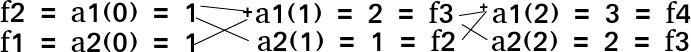
\includegraphics[width=.6\textwidth]{./pictures/12_15_1.png}
  \caption{Числа Фибоначчи}
  \label{fig:12151}
\end{figure}

Нулевой шаг индукции
$$ \begin{cases}
a_2^1 = 1 = f_1, \\
a_1^1 = 1 = f_2.
\end{cases}$$
Предположим, что формула справедлива для $t$-го шага
$$ \begin{cases}
a_2^t = f_t, \\
a_1^t = f_{t+1}.
\end{cases}$$
Проверим его для $ \left( t+1 \right) $-го шага
$$ \begin{cases}
a_2^{t+1} = a_1^t = f_{t+1}, \\
a_1^{t+1} = a_1^t + a_2^t = f_{t+1} + f_t = f_{t+2}.
\end{cases}$$
Формула верна, значит это действительно числа Фибоначчи.

По формуле Бине $k$-ое число Фибоначчи можно представить как
$$f_k =
\frac{ \phi^k}{ \sqrt{5}} =
\frac{ \left( \frac{1 + \sqrt{5}}{2} \right)^k}{ \sqrt{5}}.$$

Тогда вероятность того, что на $k$-ом шаге игра завершится равна
$$P \left( \xi = k \right) =
P \left( \eta_k = F \right) =
\frac{f_k}{2^{k-1}} \cdot \frac{1}{2} =
\frac{ \left( 1 + \sqrt{5} \right)^k}{2^{2k} \cdot \sqrt{5}} =
\frac{ \sqrt{5}}{5} \cdot \left( \frac{1 + \sqrt{5}}{4} \right)^k.$$

Найдём математическое ожидание такой случайной величины
$$M \xi =
\sum \limits_{k=2}^{ \infty } k \cdot P \left( \xi = k \right) =
\sum \limits_{k=2}^{ \infty } k \cdot \frac{ \sqrt{5}}{5} \cdot \left( \frac{1 + \sqrt{5}}{4} \right)^k =
\frac{ \sqrt{5}}{5} \sum \limits_{k=2}^{ \infty } k \left( \frac{1 + \sqrt{5}}{4} \right)^k.$$

Введём обозначения
$$ c = \frac{ \sqrt{5}}{5}, q = \frac{1 + \sqrt{5}}{4}.$$
Тогда
$$M \xi =
c \sum \limits_{k=2}^{ \infty } kq^{k}.$$

Найдём сумму
$$c \sum \limits_{k=2}^{ \infty } q^k =
c \cdot \sum \limits_{k=1}^{ \infty } q^{k-1} =
\frac{c}{q} \sum \limits_{k=1}^{ \infty } q^{k} =
\frac{c}{q} \cdot \frac{q}{1-q} =
\frac{c}{1-q}.$$

Возьмём производную от этого значения
$$c \cdot \frac{ \partial Q}{ \partial q} =
c \cdot \frac{ \partial }{ \partial q} \left( \frac{1}{1-q} \right) =
\frac{c}{ \left( 1-q \right)^2}.$$

Далее нужно подставить значения $с$ и $q$ и взять целую часть от полученного значения.

Рассмотрим более простое решение, которое даёт правильный ответ.
Приведём задачу к одномерной (рис. \ref{fig:12152}).

\begin{figure}[h!]
  \centering
  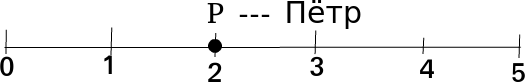
\includegraphics[width=1\textwidth]{./pictures/12_15_2.png}
  \caption{Одномерная задача}
  \label{fig:12152}
\end{figure}

Если точка $P$ попадает в точку 0, то Пётр разоряется.
Если точка $P$ оказывается в точке 5, то Иван разоряется.

Обозначим через $f \left( x \right) $ среднее время до попадания точки $P$ в точку 0 или 5, начиная из точки $x$.

Имеем граничные условия $f \left( 0 \right) = f \left( 5 \right) = 0$.

С вероятностью $1/2$ точка $P$  переходит на следующую позицию вправо и с вероятностью $1/2$ --- влево, поэтому
$$f \left( x \right) =
\frac{1}{2} \cdot f \left( x+1 \right) + \frac{1}{2} \cdot f \left( x-1 \right) +1,$$
где единица прибавляется потому, что на переход потратили 1 шаг.

Ищем $f \left( x \right) $ в виде $f \left( x \right) = ax^2 + bx + c$.

Подставляем граничные условия, чтобы найти константы $f \left( 0 \right) = c = 0$.
Теперь $f \left( x \right) $ имеет вид $f \left( x \right) = ax^2 + bx$.
Подставляем второе граничное условие $f \left( 5 \right) = 25a + 5b = 0$.
Делим уравнение на 5.
Получаем
$$5a + b =
0.$$
Выражаем $b$ через $a$.
Получаем $b = -5a$.
Подставляем это значение в исходное уравнение $f \left( x \right) = ax^2 - 5ax$.

В нашей задаче начальная точка --- это $x = 2$.
Находим значение $f$ в точке 2
$$ \begin{cases}
f \left( 2 \right) = a \cdot 2^2 - 5 \cdot 2 a = 4a - 10a = -6a, \\
f \left( 2 \right) = \frac{1}{2} \cdot f \left( 3 \right) + \frac{1}{2} \cdot f \left( 1 \right) + 1. 
\end{cases}$$

Находим $f \left( 3 \right) = 3^2 \cdot a - 5 a \cdot 3 = 9a - 15a = -6a$ и $f \left( 1 \right) = a - 5a = -4a$.
Подставляем
$$f \left( 2 \right) =
\frac{1}{2} \cdot \left( -6a \right) + \frac{1}{2} \cdot \left( -4a \right) + 1 =
-3a - 2a + 1 =
-5a + 1.$$

Приравниваем $f \left( 2 \right) $, полученные разными способами $-6a = -5a + 1$.
Переносим $-5a$ влево $-6a + 5a = 1$.
Приводим подобные $-a = 1$.
Получаем коэффициент $a = -1$.

Из этого следует, что коэффициент $b = -5a = -5 \cdot \left( -1 \right) = 5$.

Подставляем найденные коэффициенты $a$ и $b$ в уравнение
$$f \left( x \right) =
-x^2 + 5x =
x \left( 5 - x \right).$$

Нужное нам значение --- $f \left( 2 \right) = -6a = -6 \cdot \left( -1 \right) = 6$.
Аналогично
$$f \left( 3 \right) =
-6a =
6,$$
то есть среднее количество игр до разорения одного из игроков равно шести.

\subsubsection*{12.16}

\textit{Задание.} Для борьбы с колорадским жуком было создано новое средство --- вирус AB75.
При его тестировании было обнаружено,
что если колорадский жук заразился в $n$-й день вирусом AB75,
то в следующий день он инфицирует случайное количество колорадских жуков, которое имеет распределение Пуассона с параметром
$$ \lambda_n =
\frac{10}{n},$$
и умирает.
Найдите математическое ожидание количества колорадских жуков,
которые умерли от вируса AB75 на протяжении 10 суток, если в первый день было инфицировано 4 колорадских жука.

\textit{Решение.}
